%%PREAMBLE %%%%%%%%%%%%%%%%%%%%%%%%%%%%
\documentclass[10pt, a4paper]{article}% size of txt = 10pt
\usepackage[top= 2cm,
			bottom = 2cm,
			left = 1.7cm,
			right = 1.7cm,
			footskip = 0.5cm,
			headsep = 0cm,
			headheight = 0cm
					]{geometry}
\usepackage{amsmath} % math packages
\usepackage{amsfonts}% math packages
\usepackage{amssymb} % math packages
\usepackage{graphicx} %package for including graphics
\usepackage{array}
\usepackage[thinlines]{easytable}
\usepackage{float}
\usepackage[section]{placeins}
\usepackage[hidelinks]{hyperref}
\usepackage[shortlabels]{enumitem}
\usepackage{svg}
\usepackage{bigstrut}
\usepackage{wrapfig,lipsum,booktabs}
\usepackage{subcaption}
\usepackage{xfrac}
\usepackage{pdfpages}
\usepackage{listings}
\usepackage{xcolor}


\usepackage{listings}
\usepackage{color} %red, green, blue, yellow, cyan, magenta, black, white
\definecolor{mygreen}{RGB}{28,172,0} % color values Red, Green, Blue
\definecolor{mylilas}{RGB}{170,55,241}

\definecolor{codegreen}{rgb}{0,0.6,0}
\definecolor{codegray}{rgb}{0.5,0.5,0.5}
\definecolor{codepurple}{rgb}{0.58,0,0.82}
\definecolor{backcolour}{rgb}{1,1,1}

\lstdefinestyle{mystyle}{
    backgroundcolor=\color{backcolour},   
    commentstyle=\color{codegreen},
    keywordstyle=\color{magenta},
    numberstyle=\tiny\color{codegray},
    stringstyle=\color{codepurple},
    basicstyle=\ttfamily\footnotesize,
    breakatwhitespace=false,         
    breaklines=true,                 
    captionpos=b,                    
    keepspaces=true,                 
    numbers=left,                    
    numbersep=5pt,                  
    showspaces=false,                
    showstringspaces=false,
    showtabs=false,                  
    tabsize=2
}
\lstset{style=mystyle}


%date format
\def\mydate{\leavevmode\hbox{\twodigits\day.\twodigits\month.\the\year}}
\def\twodigits#1{\ifnum#1<10 0\fi\the#1}

\usepackage{indentfirst}
\setlength{\parindent}{1cm}

\makeatletter
\newcommand{\thickhline}{%
    \noalign {\ifnum 0=`}\fi \hrule height 2pt
    \futurelet \reserved@a \@xhline
}
\newcolumntype{"}{@{\hskip\tabcolsep\vrule width 2pt\hskip\tabcolsep}}
\makeatother
\newcolumntype{?}{!{\vrule width 2pt}}
%%DOC ENVIROMENT%%%%%%%%%%%%%%%%%%%%%%%xx
\begin{document}
%Title 
\begin{flushleft}%% left justification
	\textbf{\Large{MKC-IKS: Úkol č. 3}}\hfill Filip Paul\\
	\large{Vzorkování, RF imbalance \hfill\mydate}
\end{flushleft}
	\section*{\Large Úkol 1 - Vzorkování:}
        \subsection*{Zadání:}
           Reálný pásmový signál na kmitočtu nosné 6 MHz má šířku pásma 2 MHz.
           Jakým nejmenším vzorkovacím kmitočtem jej můžeme (bez aliasingu) vzorkovat při:
           \begin{enumerate}
            \item	Vzorkování dle standardního Nyquist teorému (1bod) ?
            \item	Vzorkování pomocí tzv. pásmového vzorkování (1body) ?
            \end{enumerate}
            Pro oba případy nakreslete vhodný obrázek (1 bod)

        \subsection*{Vypracování:}
        \begin{enumerate}

            \item	\textbf{Vzorkování dle standardního Nyquist teorému:}
            \begin{figure}[ht!]
                \centering
                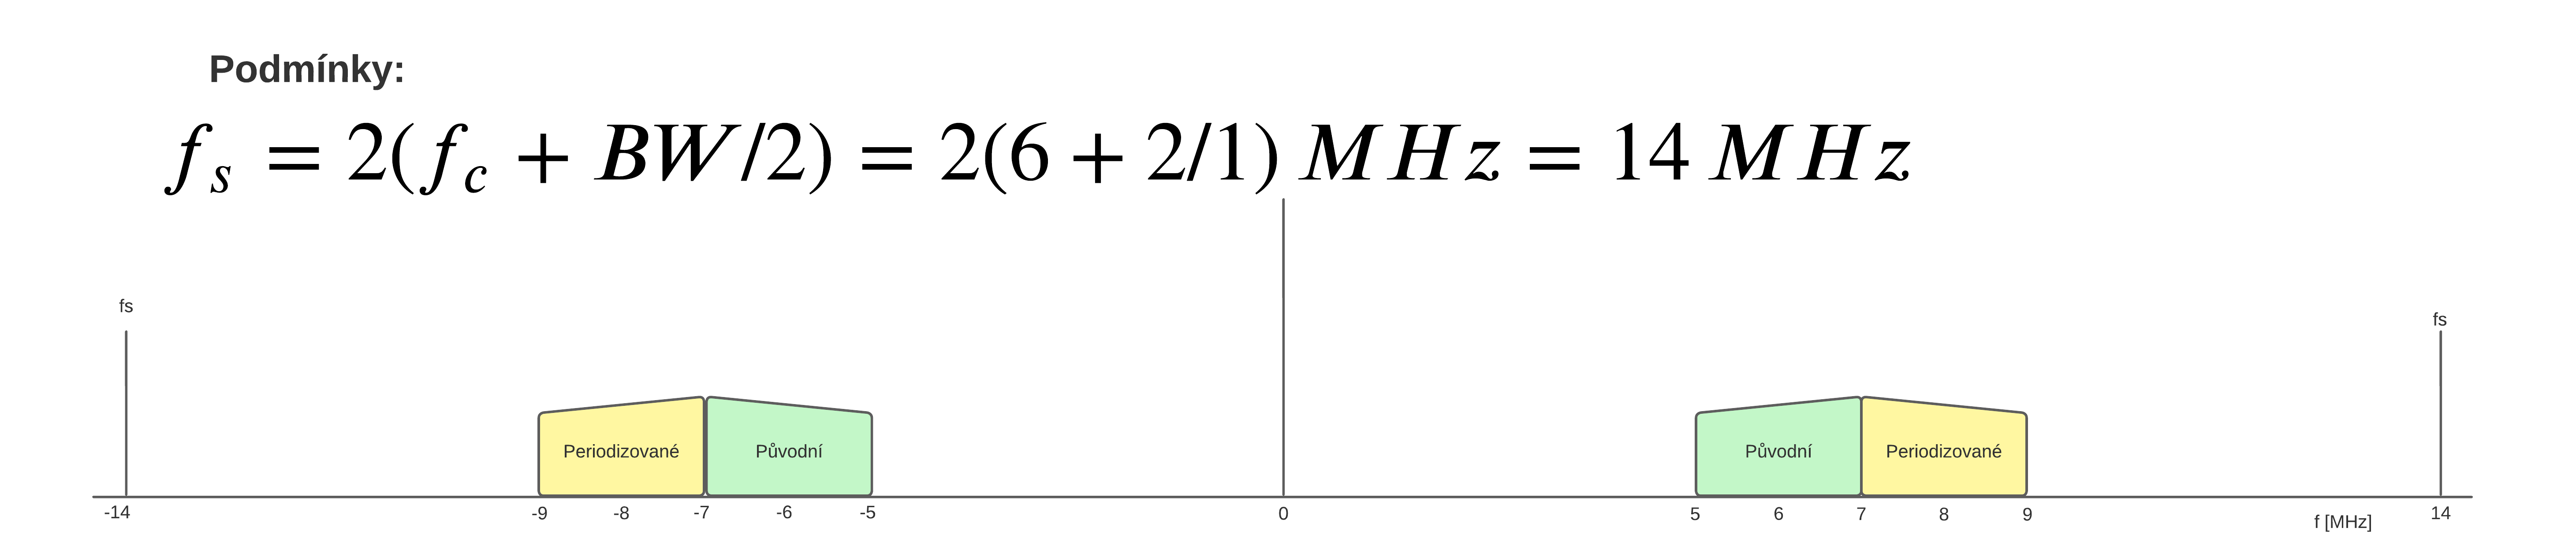
\includegraphics[width = \textwidth]{pict/NQST.png}
            \end{figure}            
            \item	\textbf{Vzorkování pomocí tzv. pásmového vzorkování:}\\
            pro tento úkol byl použit následující python script:
            \lstinputlisting[language=python]{calc.py}

            Výstupem jsou pak následující hodnoty:\\
            Awaiable intervals for k:\\
            Interval for k = 1; FS: (14.0 ; inf) MHz\\
            Interval for k = 2; FS: (7.0 ; 10.0) MHz\\
            Interval for k = 3; FS: (4.666666666666667 ; 5.0) MHz\\

            Nejnižší možná vzorkovací frekvence je tak, 4.666666666666667 MHz. Obrázek na další straně
            zobrazuje vzorkování pro fs = 5\,MHz z důvodu snažšího kreslení.

            \begin{figure}[ht!]
                \centering
                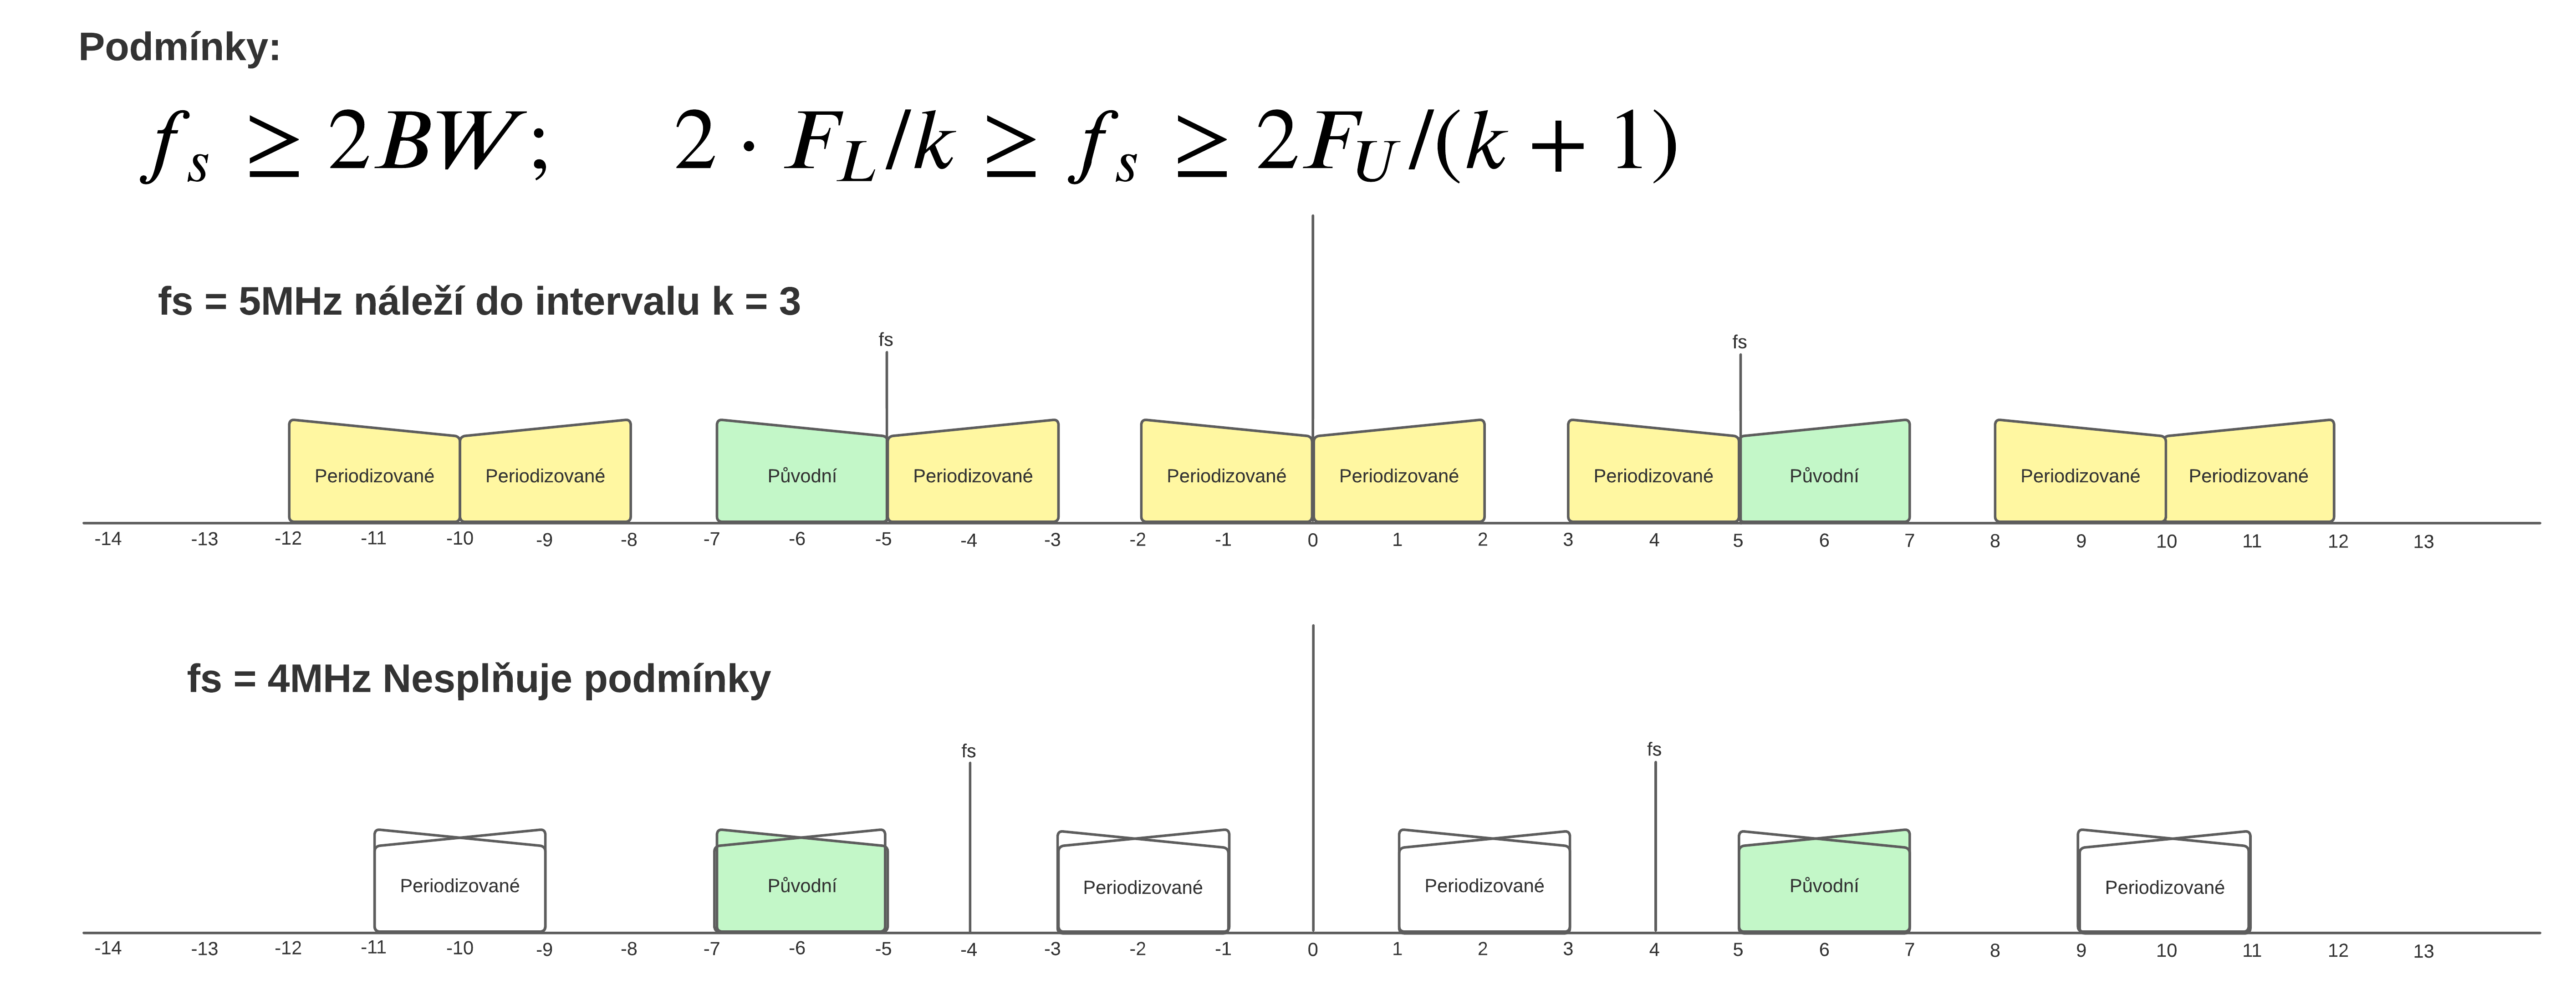
\includegraphics[width = \textwidth]{pict/BandPass.png}
            \end{figure}
            \end{enumerate}

            
    
    \section*{\Large Úkol 2 - RF imbalance:}
    \subsection*{Zadání:}
    Pro komunikační systém na bázi OFDM s dobou trvání symbolu 1$\mu$s máme na vysílací a
    přijímací straně k dispozici lokální oscilátory s nominálním kmitočtem 800 MHz a přesností (chybou)
    10ppm.  Posuďte, zda bude v tomto případě docházet k interferencím mezi nosnými OFDM v
    důsledku kmitočtového ofsetu (CFO) mezi lokálním oscilátorem vysílače a přijímače. 

    \subsection*{Vypracování:}
    Z podmínky pro ortogonalitu platí, že nosné jsou od sebe vzdáleny o 1/Ts = $1/1\mu s$ = 1\,MHz.
    Chyba 10ppm na 800\,MHz znamená frekvenční offset 8\,kHz. Což dělá cca 0.8\% ze vzdálenosti nosných OFDM.
    Nemělo by tak docházet k nějakým výrazným interferencím.





\end{document}
%\[f(x)= (x+2)^2 - \frac{9\cdot 2\pi}{26}\] %%mathematic equatation in display style mode
%%optional:
%	\begin{align} %%this alignes all charakters after & if *is removed equations will be numbered
%	\hspace{5cm}  
%		 x &= a_2 x^2 +_1 x + a_0 \\
% 		x &=x^2 \nonumber		%no number will not add number to eq
%	\end{align}